\clearpage
\section{Indledning}
%Introduktion til TV2
Dette semesters projekt tager udgangspunkt i TV 2 og deres måde at håndtere krediteringer på. TV 2 er en dansk tv-station, der blev grundlagt i 1988. TV 2's forretning og den måde de tjener deres penge på, fungerer ved at lave kvalitetsbevidst tv til de danske stuer. TV 2 gør deres tv-kanaler tilgængelige hos forskellige tv-udbydere, oveni at de viser reklamer mellem deres programmer, som skaber deres primærer indkomst, sammen med indtægterne fra abonnenter på deres streamingtjenseste TV 2 Play.

%TV2's plads på markedet
TV 2 er, ligesom alle andre tv-produktioner, en del af et stort marked, hvor tv-skærmen er deres vindue ud til forbrugeren. På sådanne et marked handler det om at få seeren til at bruge mere tid på sine egne kanaler, frem for konkurrentens. Hvis man vil holde styr på konkurrencen mellem kanalerne, vil det nemmeste nok være at kigge på, hvor mange seere der er på en given kanal, og hvor mange minutter seeren bruger på kanalen. Ud fra Kantars seereundersøgelser kan alle og enhver se seertallene på de forskellige tv-kanaler. Kantar indsamler nemlig seeretal hvert sekund, for at kunne levere de mest præcise seeretal \cite{url_kantar}, som programlæggere i tv-branchen bruger til at forbedre tv-oplevelsen for seerene, og fastlægge hvilke tider i sendefladen, der er mest værdifulde. I følgende figur, som både er tilgængelig på Kantars hjemmeside, men også i vores case fra TV 2 af, kan man se hvor mange minutter TV 2s kanaler bliver set i forhold til de andre tv-kanaler.
\begin{figure}[H]
    \centering
    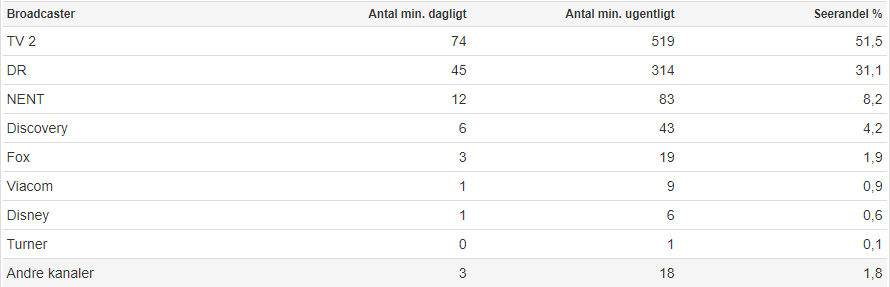
\includegraphics[width=1\textwidth]{images/Seertal.png}
    \caption{Seertid i uge 3 2020}
    \label{fig:Seertid}
\end{figure}
Det første tal der ses i figur \ref{fig:Seertid} viser, hvor mange minutter den gennemsnitlige dansker bruger på en given udbyders tv-kanaler. Det næste tal viser hvor mange minutter det er om ugen, og det sidste tal viser, hvor stor en seerandel den givne udbyder besidder på markedet for perioden. \\
%Problemet
Som det ses har TV 2 en stor seerandel, og af den grund består en vigtig del af deres indkomst af de reklamer de sender mellem deres programmer.  Men den indkomst kan blive bedre endnu, hvis de bliver bedre til at optimere tiden mellem deres programmer, vurderer TV 2. Og det er netop dette problem som danner grundlag for vores case.

\subsection{Redegørelse for den udleverede case}
Når et program slutter på en af TV 2s kanaler, bliver der vist rulletekster for at kreditere de medvirkende i programmet. Disse rulletekster tager dog i nogle tilfælde op til 30 sekunder, hvilket er 30 sekunder for meget. TV 2 har vurderet, at hvis man kan frigøre disse 30 sekunder fra rulleteksterne, og bruge dem på reklamer i stedet, vil det kunne give dem en øget indtægt på op imod 60 millioner kroner om året. \cite{url_case}

Netop dette vil TV 2 gøre ved at digitalisere krediteringerne, så de kan ses på nettet eller en applikation. For Udover at kunne sende flere reklamer mellem deres programmer, vil TV2 også have muligheden for at kreditere alle, og ikke bare de vigtigste efter endt program. I de fleste tilfælde er 30 sekunders rulletekster nemlig ikke nok til at kreditere alle medvirkende, så derfor har TV2 været nødt til at prioritere, hvilket selvfølgelig fører til at nogle krediteringer bliver glemt. Digitaliseres krediteringerne, vil alle kunne blive krediteret ligeligt, og der vil derved ikke være nogen som bliver glemt, fordi deres rolle i produktionen er mindre vigtig.

Vores opgave i denne case er at skabe netop denne digitalisering af krediteringer. Det er vores opgave at udvikle et software system, som kan tilføje, fjerne og redigere krediteringer i en database, hvortil vi har formuleret en problemformulering, som skal hjælpe os med at få udarbejdet en løsning på TV 2s problematik med kreditering.

\subsection{Formålet med opgaven}
Formålet med det system vi udvikler, er at gøre det lettere for producere, administratorer og TV2 som virksomhed, at kunne redigere og holde styr på krediteringer. Derudover er formålet med projektopgaven også at vi som gruppe skal forbedre vores evner inden for programmering af softwaresystemer og håndtering af databaser. Samtidigt med at vi videre udvikler vores kompetencer inden for gruppearbejde, og opsætning af et struktureret arbejdsmiljø.

Vores semesterprojekt er inddelt i flere dele; først og fremmest har vi vores "inception", altså første del. Denne del gik ud på at få udarbejdet et inceptionsdokument, som skulle lægge et fundament for vores videre arbejde med projektet. Formålet med dette inceptionsdokument var at vi som gruppe skulle ende med et veldefineret projektgrundlag, som indebar at der var styr på krav, scope og problemformuleringen. Udover dette skulle vi også klargøre, hvilke metoder vi ville benytte os af, for at kunne løse den problemformulering vi havde sat os for.

Efter inceptionen har vi den faktiske løsning af projektets problemformulering. Her har vi undersøgt og besvaret de spørgsmål vi satte os for i problemformuleringen, samt benyttet os af vores forarbejde i første del af projektet til at kunne udvikle koden effektivt.\\
Fordelen med at have delt vores projekt op i flere dele, har været at vi som gruppe i første del har kunne skabe os en forståelse for hvad problemet er, hvordan vi vil gribe casen an og hvordan vi som gruppe vil løse problemet på den bedst mulige måde. Dertil har vi så efterfølgende, senere hen i projektet, kunne fokusere på at følge vores planer og benytte vores forarbejde, til at udvikle det bedst mulige softwaresystem, og besvare problemformuleringen.

\subsection{Problemanalyse}
For at gå i dybden med den stillede case fra TV 2, og dermed vurdere hvad det essentielle problem er, samt skabe os en problemformulering til at arbejde ud fra, har vi først analyseret casen, med fokus på at identificere, hvilke mulige problemer der er. Den case som TV 2 har lavet, er relativt udpenslet, og der er ikke meget tvivl om, at det essentielle problem for dem er, at det er for besværligt at håndtere krediteringer til produktioner på den måde, som de gør i øjeblikket, nemlig at synliggøre krediteringer i 30 sekunder efter endt program i form af rulletekster. Denne nuværende løsning er et problem, da 30 sekunder ikke er nok til at kunne vise alle medvirkende i nogle udsendelser. \cite{url_case} Der er også flere regler, som skal overholdes når der vises rulletekster, som f.eks:
\begin{itemize}
    \item Ophavsretsloven
    \item TV 2s overenskomster
    \item Kontrakter for ophavsmænd og udøvende kunstnere
    \item Almindelig god skik
\end{itemize}
Ud fra de informationer vi har erhvervet os fra casen omkring TV 2s regler for hvad og hvordan der skal angives krediteringer, har vi skabt et problem træ, der skal visualisere hvordan vi ser dette problem. Dette problemtræ ses i figur \ref{fig:problemtræ}. 

Kigger man på problemtræet, vil man kunne se, at de 30 sekunder, som der maksimalt må vises rulletekster i, skaber nogle problemer for TV 2. TV 2 mister nemlig skærmtid, af at skulle vise rulletekster efter hvert program, men udover det, har de, som tidligere nævnt, svært ved at få plads til samtlige krediteringer på 30 sekunder. Vi vurderer derfor at årsagen, bag disse problemer er, at TV 2 er begrænset til at vise krediteringer i tv'et, og dette problem kan løses ved at flytte krediteringer over på et andet medium end tv-skærmen. 

 \begin{figure}[H]
    \centering
    \begin{tikzpicture}[grow'=up]
        \tikzset{level distance=42pt}
        \Tree [ .{30 sekunder til rulletekster} 
                [.{Prioritering af krediteringer}
                    [.{Inkorrekt kreditering}
                        [.{Brud på ophavsretslov} 
                            [.{Brud på overenskomster\\og andre aftaler} ] ]
                    ]
                ]
                [.{Tab af skærmtid}
                    [.{Mindre reklamer} 
                        {Dårligere omsætning\\(tab på 60 mio. kr.)} 
                    ] 
                    [.{Mindre programtid} 
                        {Dårligere seeroplevelse} 
                    ] 
                ]
            ] 
        \tikzset{grow'=down}
        \Tree [ .{\\} 
                [.{Krediteringer vises på TV-skærm} 
                    [.{Tilgængelighed for alle} ]
                    [.{Der findes ikke nogen online\\alternativ til kreditering\\af danske produktioner} ]
                ]
            ]
              
    \end{tikzpicture}
    \caption{Problemtræ omkring de informationer, der er givet i casen.}
    \label{fig:problemtræ}
\end{figure}

\subsection{Problemformulering}
Ud fra vores analyse af TV 2s case, er vi kommet frem til en problemformulering og dertilhørende underspørgsmål. Vores problemformulering har vi formuleret således:\\
\linebreak
\textbf{Hvordan kan vi udvikle en prototype til et krediteringssystem, der vil kunne erstatte de klassiske rulletekster efter et afsluttet program?}
\\\\
Og vores underspørgsmål, til at supplere problemformuleringen lyder således:
\begin{itemize}
    \item Hvordan er reglerne for krediteringer for danskproducerede programmer?
    \item Hvilke informationer skal og må inkluderes i krediteringer?
    \item Hvordan kan sådan et program gøres mest mulig brugervenligt for både seer og administrator?
    \item Hvordan kan vi sikre et velstruktureret program, der mindsker fejl og ventetid, samt strukturere databasen således, at der undgås fejl, duplikering af værdier og null-værdier?
\end{itemize}

\subsection{Afgrænsninger}
Projektet kan blive stort, og der er et utal af muligheder for, hvordan man kan skabe en overskuelig softwareløsnign på TV2 s problem. Derfor har det også været vigtigt for os, at begrænse os. Vi vil gerne undgå at bruge for meget tid på, funktionalitet, som ikke er vigtig, og lægge vores kræfter i de ting, som vi ved, vi kan overskue at gennemføre, og som der er tid til at få udviklet. Efter et interview med Morten Lehm fra TV 2, blev der oplyst, at det ikke er muligt at inddrage ikke-danske produktioner i softwaresystemet (se bilag \ref{kundemøde} ), og gruppen holder sig derfor til, udelukkende at arbejde med danske krediteringer, og undgår derved bevidst krediteringer til udenlandske shows og programmer.
Gruppens produkt udarbejdes også kun som en prototype, og det betyder, at produktet ikke vil blive udviklet til et færdigt produkt, som vil opfylde alle givne krav fra TV 2s side af. Krediteringerne vil dog stadig overholde de givne regler for krediteringer, men kommer til slut ikke til at være et produkt TV 2 kan adaptere direkte over til. 
